\begin{figure}[!t]
    \centering
    \subfloat{
        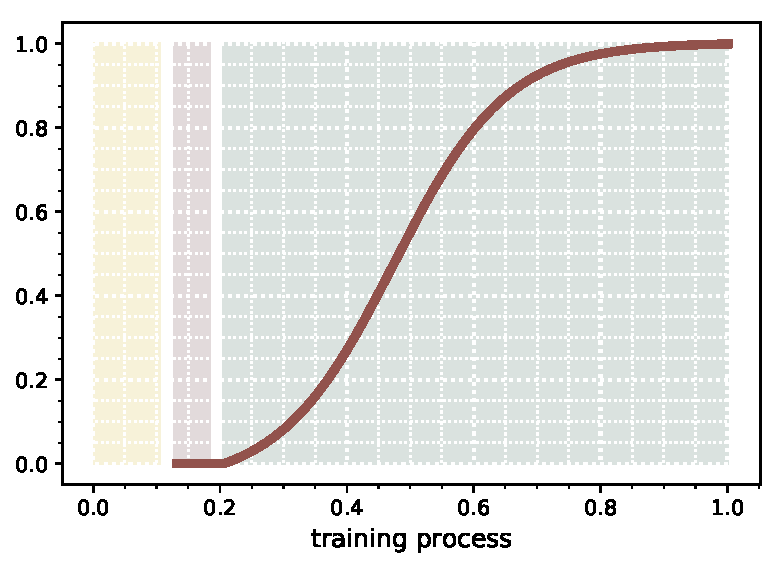
\includegraphics[width=0.4\textwidth]{contents/figures/pdf/analysis/TransferabilityOffset.pdf}
    } 
    \\
    \hspace{0mm}
    \subfloat{
        
\includegraphics[width=0.32\textwidth]{contents/figures/pdf/analysis/annotation.pdf}
        } 
    \caption{
        The changing of $\gamma$ with $\gamma_0=1$. 
        We use three different color to denote three different training stage $N_0, N_1$ and $N_2$. 
        In particular, $N_0$ is the pretrain stage on the source domain, thus $\sigma$ is not used. 
        In the stage of $N_1$, $\gamma$ is set to be $0$ so as to select most transferable samples. 
        In stage $N_2$, the $\gamma$ progressively grows according to $\sigma(\cdot)$.
    }
    \label{figure: offset changing}
\end{figure}